\section*{\fontsize{25}{29}\selectfont{\textbf Contribution} \\}

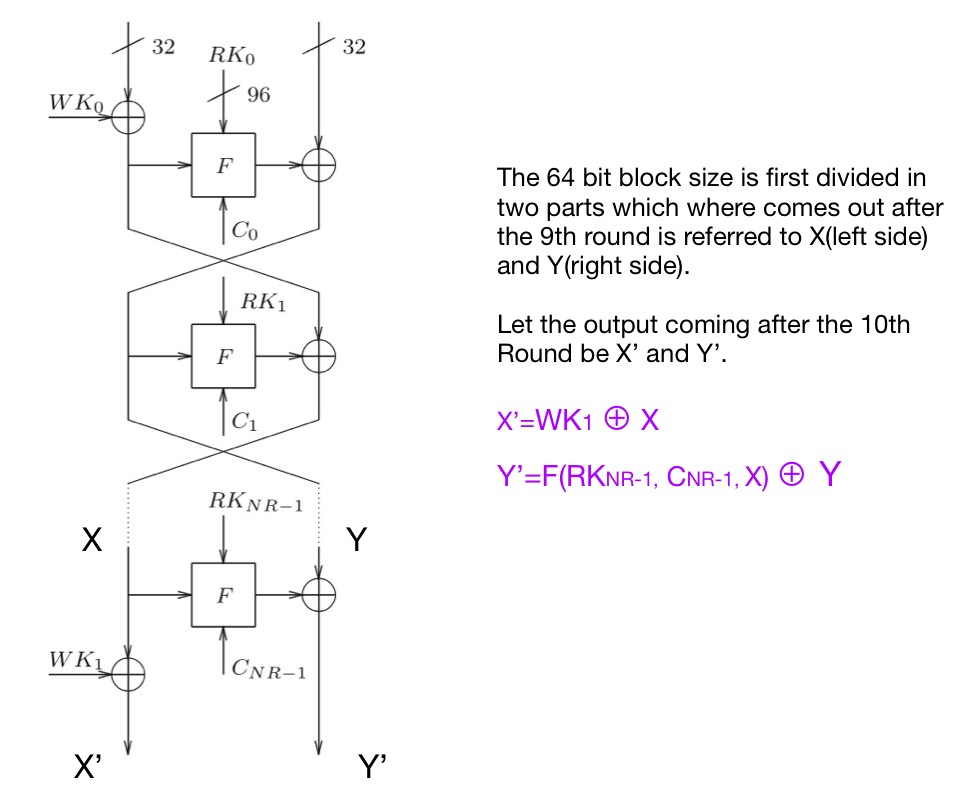
\includegraphics[scale=0.5]{project/images/7.jpg}

Now the equations 1 and 2 came when we have not induced any fault at any step.

Now let us put a fault after the 9th round such that Y becomes Y1.

Now the perceived output show some change and let the new output be Y1’.

Now the change in equation is :

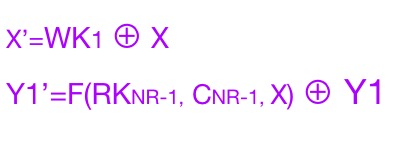
\includegraphics[scale=0.5]{project/images/8.jpg}

Here the known variables are X’ ,Y’ and Y1’
and unknown variables are X,Y,X’,Y’,WK1
Now we are working on to solve 5 unknown variables and We are exploring the function F and we are also trying to reduce the  fair complexity in decrypting the function F. We have 3 equations and from this we will try to decipher the key using some mathematical operations on the equations.

Now we are doing Faults:\\

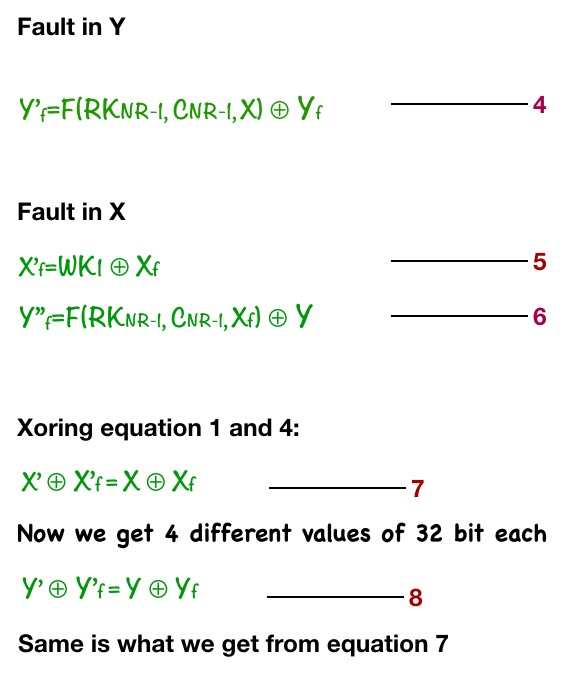
\includegraphics[scale=0.7]{project/images/9.jpg}

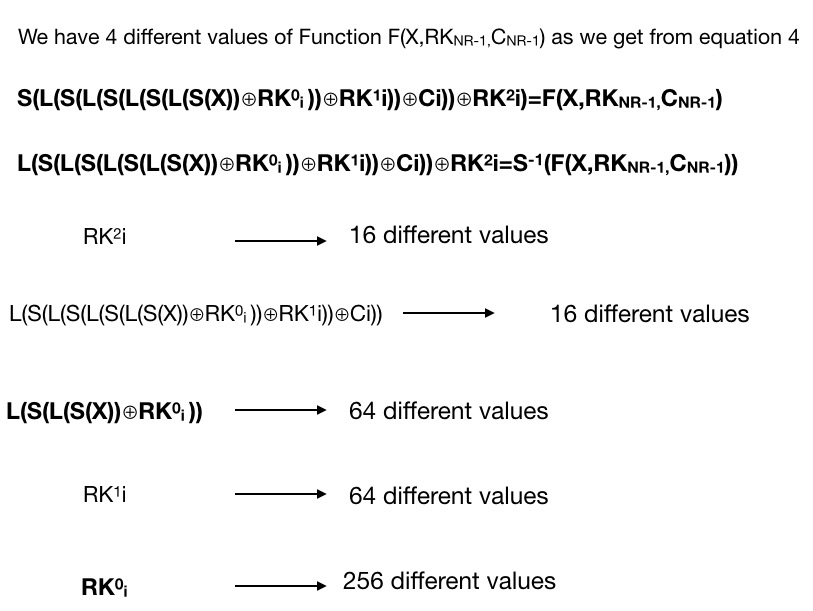
\includegraphics[scale=0.60]{project/images/10.jpg}


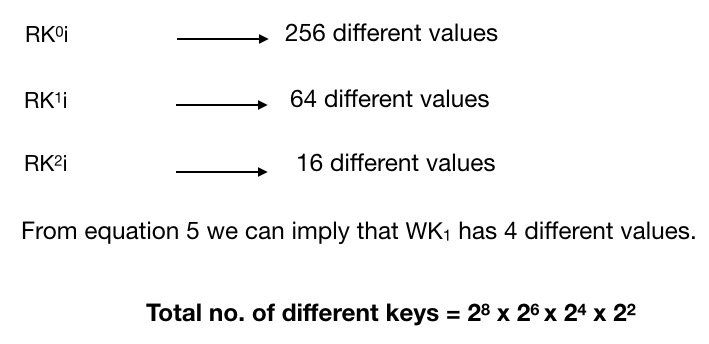
\includegraphics[scale=0.70]{project/images/11.jpg}

Now we reduce the exhaustive search space for possible keys of RoadRunneR:

\hspace{3.5cm}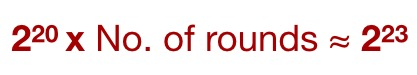
\includegraphics[scale=0.60]{project/images/12.jpg}

